%%%%%%%%%%%%%%%%%%%%%%%%%%%%%%%%%%%%%%%%%%%%%%%%%%%%%%%%%%%%%%%%%%%%%%%
%% Zusammenfassung und Ausblick
\section{Entwicklung}
\label{sec:entwicklung}
Dieses Kapitel befasst sich mit einzelnen Aspekten der Entwicklung. Nach der anfänglichen Anforderungsanalyse werden grundlegende Konzepte und Architekturen vorgestellt. Dabei werden erste Sensoren, Aktoren und bestehende Software Bibliotheken getestet und für eine Anschlussverwendung bewertet. Die weiteren benötigten Softwarepaket werden im nachfolgenden Kapitel Implementierung umgesetzt.


\subsection{Anforderungsanalyse}
In diesem Kapitel werden die Anforderungen an das Robotersystem gestellt. Es werden die einzelnen Funktionalitäten für die Aktoren und Sensoren festgelegt. Außerdem werden die Anforderungen an die Architektur definiert. Das folgende Use-Case Diagramm \ref{fig:dev-usecase} stellt die groben Funktionsanforderungen an das Roboter System dar.

 \begin{figure}[H]
 	\centering
 	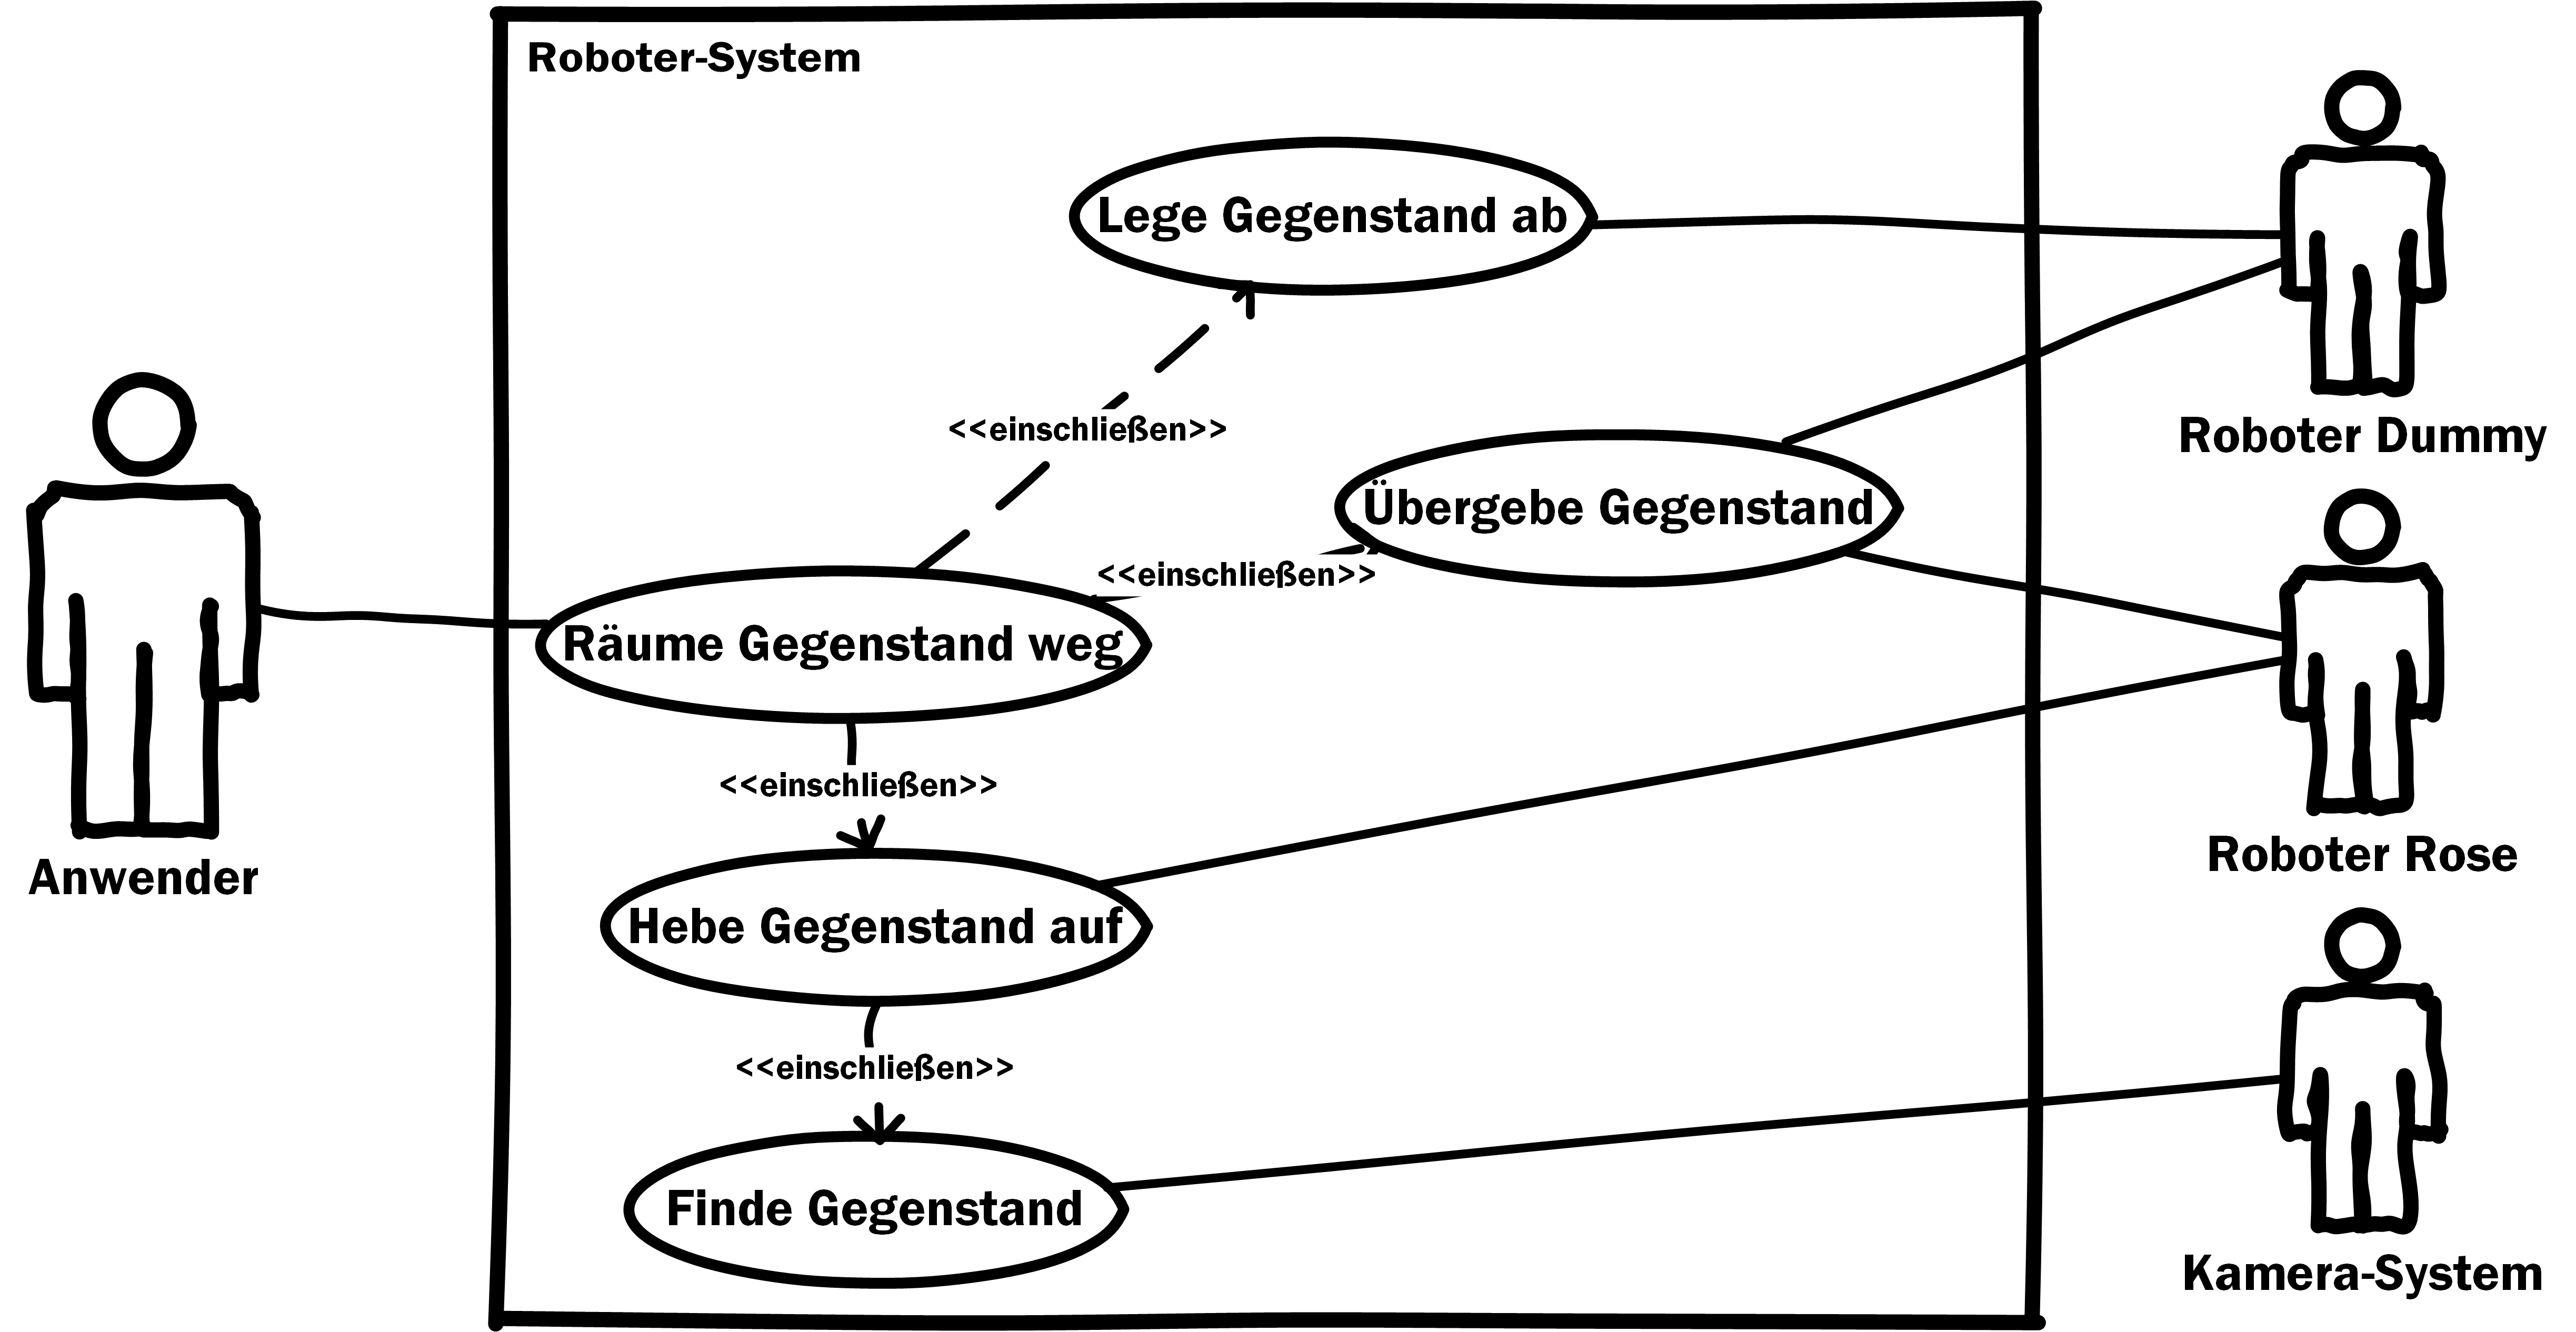
\includegraphics[scale=0.8]{fig/UseCase}   
 	\caption[Use-Case Robotersystem]{Vereinfachtes Use-Case Diagramm zur groben Funktionsübersicht des Robotersystems}
 	\label{fig:dev-usecase}
 \end{figure}
 
 Der Anwender gibt dem System die Anweisung einen Gegenstand wegzuräumen. Das Robotersystem gliedert die Anweisung in einzelne Tasks auf. Diese Tasks werden von den unterschiedlichen Akteuren mit ihren Funktionalitäten sequentiell oder parallel ausgeführt. In diesem konkreten Fall soll zunächst der Roboter Rose den entsprechenden Gegenstand aufheben. Dies erfordert zunächst eine Lokalisierung des Objektes die von einem Kamerasystem angefordert wird. Anschließend übergeben sich die Roboter Rose und Dummy den Gegenstand, bevor Dummy ihn anschließend an einer gewünschten Position ablegt. Diese sehr grobe Darstellung des Vorgangs beinhaltet die vier zentralen Funktionen, die das System umsetzen muss: Gegenstand aufheben (\textit{pick-up}), Gegenstand ablegen (\textit{place}), Gegenstand lokalisieren und Gegenstand übergeben(\textit{handover}). Des Weiteren muss es eine Möglichkeit für den Anwender geben Befehle an das System zu übergeben. Diese funktionalen Anforderungen werden im nächsten Unterkapitel \ref{sec:dev-funk} aufgelistet und definiert. Neben diesen funktionalen Anforderungen existieren noch nicht-funktionale Anforderungen. Zu diesen zählen Sicherheitsaspekte, sowie Anforderungen an die Zuverlässigkeit, Erweiterbarkeit und die Effizienz. Die nicht-funktionalen Anforderungen werden in Kapitel \ref{sec:dev-nichtfunk} aufgeführt.
 
\subsubsection{Funktionale Anforderungen}
\label{sec:dev-funk}
In der Arbeit \cite{lundh2006plan} 

\subsubsection{Nicht-Funktionale Anforderungen}
\label{sec:dev-nichtfunk}

\subsection{Inverse Kinematik}
\subsection{Architektur RATS}
